\section{Parte 03 – Instalacion de Windows Server} 

\begin{enumerate}[1.]
	\item Para virtual izar nuestro Windows Server 2012 R2, haremos uso de VMWare Workstation Pro, asignando una instalación Custom

	\begin{center}
	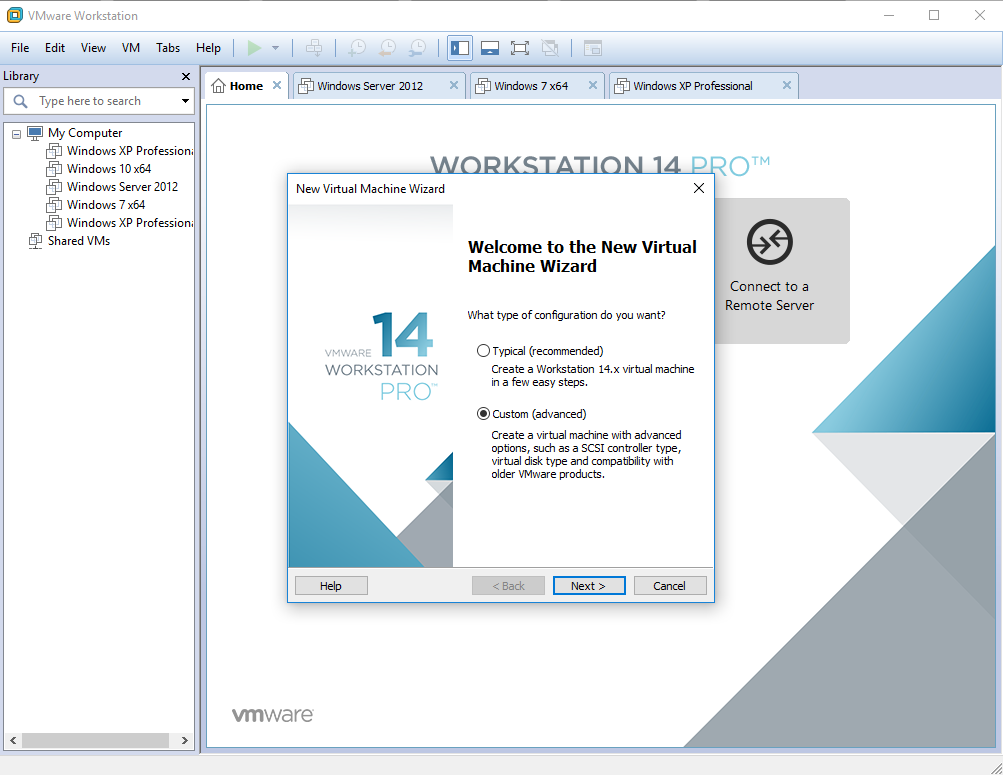
\includegraphics[width=15cm]{./Imagenes/img1server} 
	\end{center}
	
	\item Seleccionamos la tercera opción que nos permite asignar un sistema operativo después

	\begin{center}
	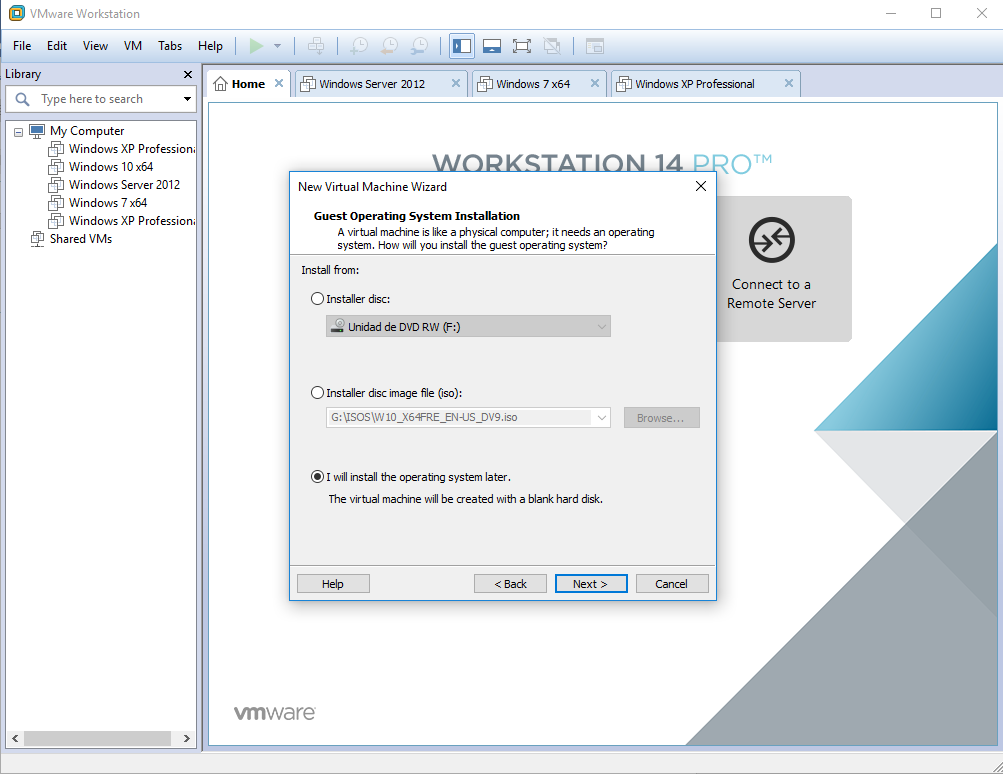
\includegraphics[width=15cm]{./Imagenes/img2server} 
	\end{center}


	\item Seleccionamos la opcion windows y buscamos en la lista Windows Server 2012

	\begin{center}
	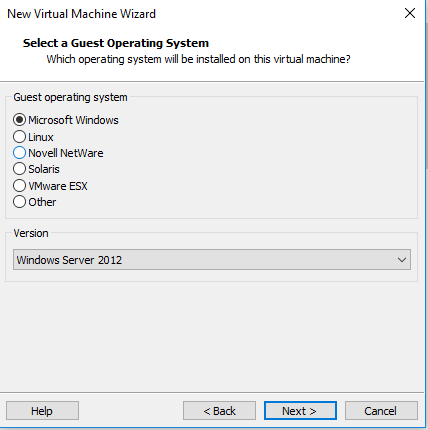
\includegraphics[width=15cm]{./Imagenes/img3server} 
	\end{center}
	
	\item Asignamos un nombre a la maquina virtual y una direccion en donde se instalara

	\begin{center}
	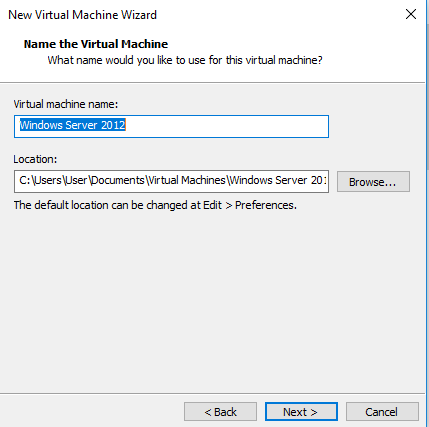
\includegraphics[width=15cm]{./Imagenes/img4server} 
	\end{center}


	\item Seleccionamos la memoria que tendra la maquina virtual

	\begin{center}
	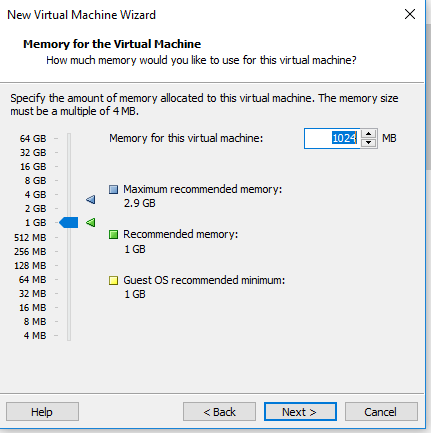
\includegraphics[width=15cm]{./Imagenes/img5server} 
	\end{center}
	
	\item Comenzamos la Instalacion

	\begin{center}
	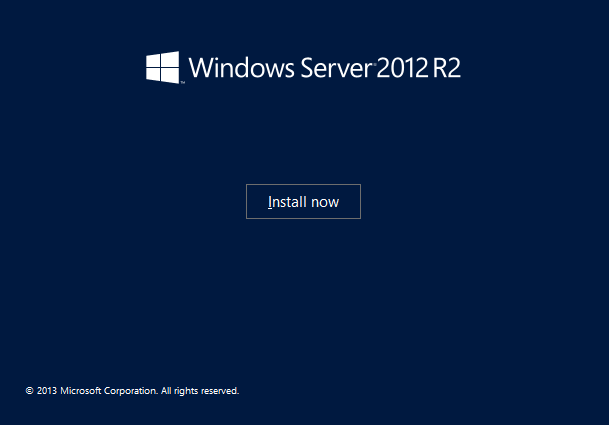
\includegraphics[width=15cm]{./Imagenes/img6server} 
	\end{center}


	\item Seleccionamos la opcion GUI

	\begin{center}
	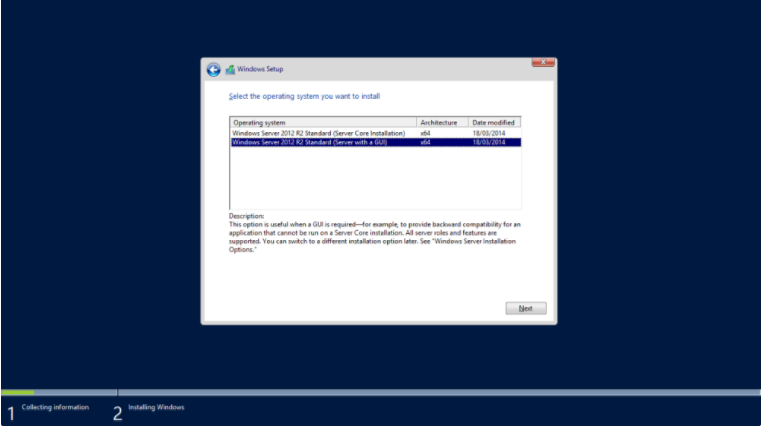
\includegraphics[width=15cm]{./Imagenes/img7server} 
	\end{center}


	\item Asignamos la contraseña Epis2018. El Administrador lo dejamos como esta

	\begin{center}
	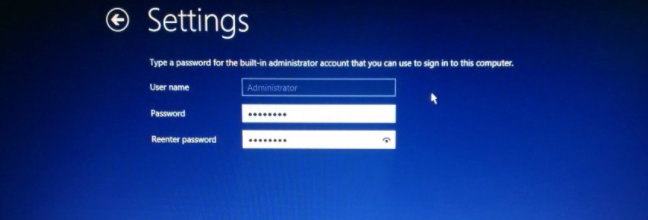
\includegraphics[width=15cm]{./Imagenes/img8server} 
	\end{center}
	
	\item siguiente paso

	\begin{center}
	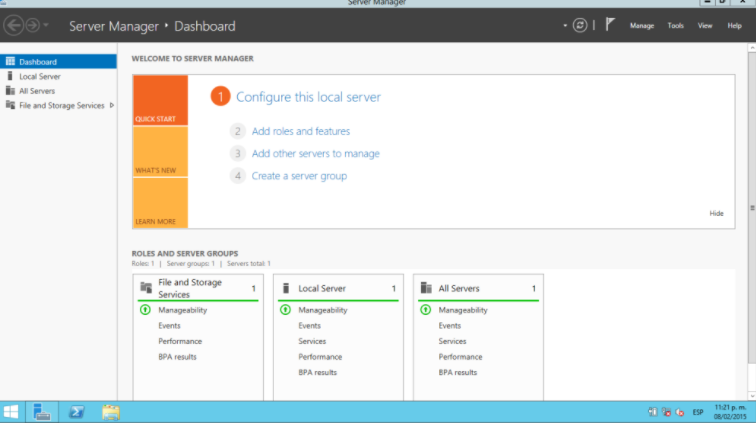
\includegraphics[width=15cm]{./Imagenes/img9server} 
	\end{center}


	\item En este laboratorio se asignará una IPv4 a cada sistema operativo para después mediante el cmd hacer ping y demostrar que están conectados.
	\subitem a)	Windows Server 2012 R2

	\begin{center}
	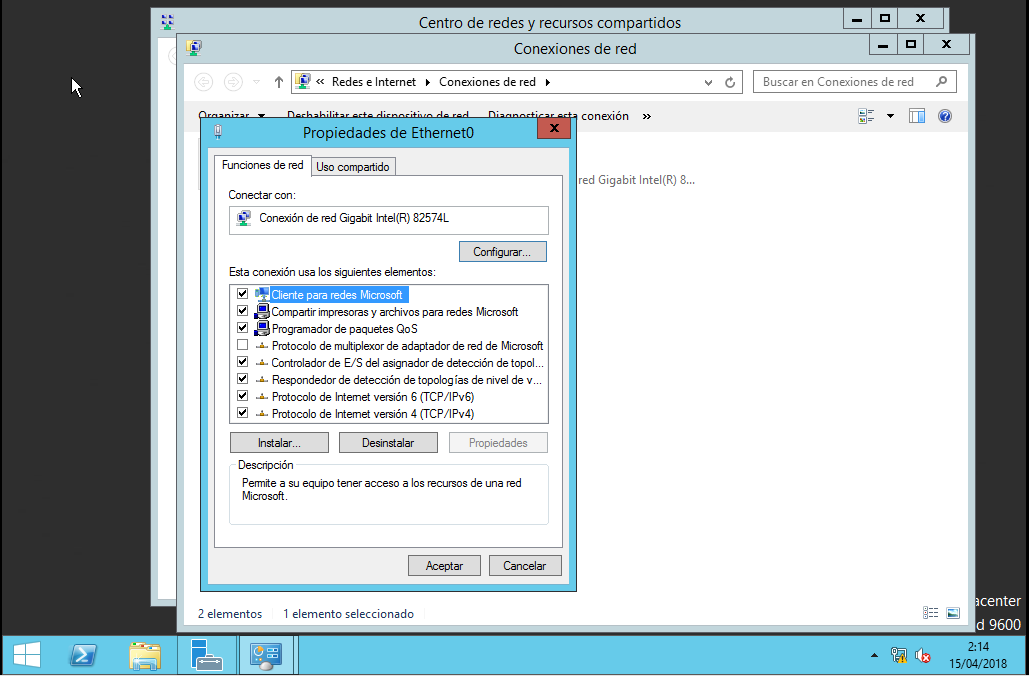
\includegraphics[width=15cm]{./Imagenes/img10server} 
	\end{center}
	
	\item Le asignamos la dirección IP que corresponde a cada estudiante determinado por el docente.

	\begin{center}
	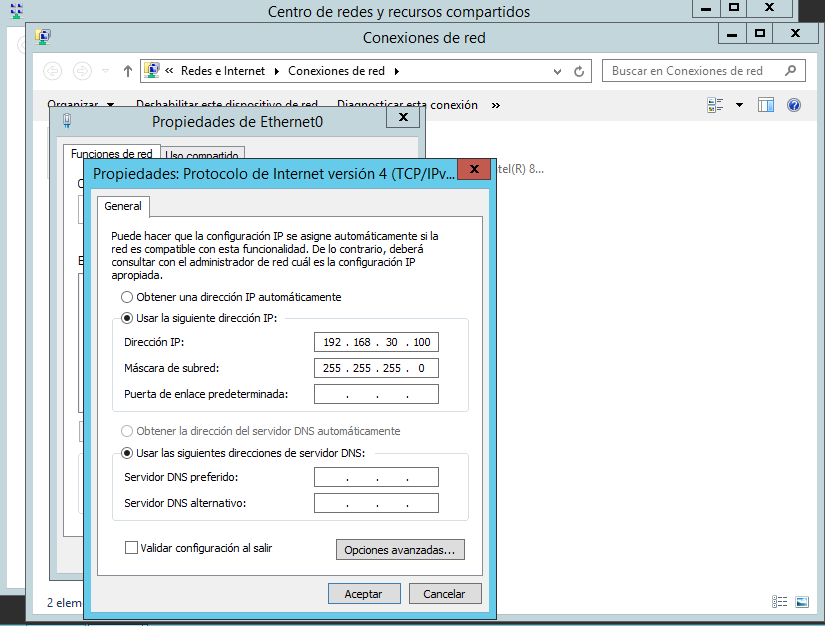
\includegraphics[width=15cm]{./Imagenes/img11server} 
	\end{center}


								

	

\end{enumerate} 
